% This is "sig-alternate.tex" V2.0 May 2012
% This file should be compiled with V2.5 of "sig-alternate.cls" May 2012
%
% This example file demonstrates the use of the 'sig-alternate.cls'
% V2.5 LaTeX2e document class file. It is for those submitting
% articles to ACM Conference Proceedings WHO DO NOT WISH TO
% STRICTLY ADHERE TO THE SIGS (PUBS-BOARD-ENDORSED) STYLE.
% The 'sig-alternate.cls' file will produce a similar-looking,
% albeit, 'tighter' paper resulting in, invariably, fewer pages.
%
% ----------------------------------------------------------------------------------------------------------------
% This .tex file (and associated .cls V2.5) produces:
%       1) The Permission Statement
%       2) The Conference (location) Info information
%       3) The Copyright Line with ACM data
%       4) NO page numbers
%
% as against the acm_proc_article-sp.cls file which
% DOES NOT produce 1) thru' 3) above.
%
% Using 'sig-alternate.cls' you have control, however, from within
% the source .tex file, over both the CopyrightYear
% (defaulted to 200X) and the ACM Copyright Data
% (defaulted to X-XXXXX-XX-X/XX/XX).
% e.g.
% \CopyrightYear{2007} will cause 2007 to appear in the copyright line.
% \crdata{0-12345-67-8/90/12} will cause 0-12345-67-8/90/12 to appear in the copyright line.
%
% ---------------------------------------------------------------------------------------------------------------
% This .tex source is an example which *does* use
% the .bib file (from which the .bbl file % is produced).
% REMEMBER HOWEVER: After having produced the .bbl file,
% and prior to final submission, you *NEED* to 'insert'
% your .bbl file into your source .tex file so as to provide
% ONE 'self-contained' source file.
%
% ================= IF YOU HAVE QUESTIONS =======================
% Questions regarding the SIGS styles, SIGS policies and
% procedures, Conferences etc. should be sent to
% Adrienne Griscti (griscti@acm.org)
%
% Technical questions _only_ to
% Gerald Murray (murray@hq.acm.org)
% ===============================================================
%
% For tracking purposes - this is V2.0 - May 2012

\documentclass{sig-alternate}
\usepackage{fixltx2e}
\usepackage{xcolor}
\usepackage{amsmath,array}
\usepackage{multirow}
\newcolumntype{L}[1]{>{\raggedright\arraybackslash}m{#1}}
\def\SPSB#1#2{\rlap{\textsuperscript{\textcolor{red}{#1}}}\SB{#2}}
\def\SP#1{\textsuperscript{\textcolor{black}{#1}}}
\def\SB#1{\textsubscript{\textcolor{black}{#1}}}
\newenvironment{myquote}
               {\list{}{\rightmargin   \leftmargin
                        \parsep        0in }%
                \item\relax}
               {\endlist}
\newcommand{\userquote}[2]{\begin{samepage}\begin{myquote} 
     \em{\small{#2\begin{flushright}---#1\end{flushright}}}
   \end{myquote}\end{samepage}}
%Quote code
%\newif\ifquoteopen
%\catcode`\"=\active % lets you define `"` as a macro
%\DeclareRobustCommand*{"}{%
%   \ifquoteopen
%     \quoteopenfalse ''%
%   \else
%     \quoteopentrue ``%
%   \fi
%}

%End of quote code
\usepackage{float}
\begin{document}
%\setlength{\parindent}{0pt}
\CopyrightYear{2016}
\setcopyright{acmcopyright}
\conferenceinfo{ACM DEV '16,}{November 17-22, 2016, Nairobi, Kenya}
\isbn{978-1-4503-4649-8/16/11}\acmPrice{\$15.00}
\doi{http://dx.doi.org/10.1145/3001913.3001920}
%
% --- Author Metadata here ---
%\conferenceinfo{ICTD'16}{June 3-6 2016, Ann Arbor, Michigan, USA}
%\CopyrightYear{2007} % Allows default copyright year (20XX) to be over-ridden - IF NEED BE.
%\crdata{0-12345-67-8/90/01}  % Allows default copyright data (0-89791-88-6/97/05) to be over-ridden - IF NEED BE.
% --- End of Author Metadata ---

%\title{Alternate {\ttlit ACM} SIG Proceedings Paper in LaTeX
%\title{Leveraging on Families' Social Interactions on Utilization of Personal Health Informatics through Intermediaries}
\title{A Family Health App: Engaging Children to Manage Wellness of Adults}
%
% You need the command \numberofauthors to handle the 'placement
% and alignment' of the authors beneath the title.
%
% For aesthetic reasons, we recommend 'three authors at a time'
% i.e. three 'name/affiliation blocks' be placed beneath the title.
%
% NOTE: You are NOT restricted in how many 'rows' of
% "name/affiliations" may appear. We just ask that you restrict
% the number of 'columns' to three.
%
% Because of the available 'opening page real-estate'
% we ask you to refrain from putting more than six authors
% (two rows with three columns) beneath the article title.
% More than six makes the first-page appear very cluttered indeed.
%
% Use the \alignauthor commands to handle the names
% and affiliations for an 'aesthetic maximum' of six authors.
% Add names, affiliations, addresses for
% the seventh etc. author(s) as the argument for the
% \additionalauthors command.
% These 'additional authors' will be output/set for you
% without further effort on your part as the last section in
% the body of your article BEFORE References or any Appendices.

\numberofauthors{3} %  in this sample file, there are a *total*
% of EIGHT authors. SIX appear on the 'first-page' (for formatting
% reasons) and the remaining two appear in the \additionalauthors section.
%
\author{
% You can go ahead and credit any number of authors here,
% e.g. one 'row of three' or two rows (consisting of one row of three
% and a second row of one, two or three).
%
% The command \alignauthor (no curly braces needed) should
% precede each author name, affiliation/snail-mail address and
% e-mail address. Additionally, tag each line of
% affiliation/address with \affaddr, and tag the
% e-mail address with \email.
%
% 1st. author
\alignauthor
        Ntwa Katule \\
        \affaddr{University of Cape Town}\\
        \affaddr{Department of Computer Science}\\
        \affaddr{Cape Town, South Africa}\\
        \email{katulentwa@gmail.com}\\
% 2nd. author
\alignauthor Ulrike Rivett\\
        \affaddr{University of Cape Town}\\
        \affaddr{Department of Information Systems}\\
        \affaddr{Cape Town, South Africa}\\
        \email{ulrike.rivett@uct.ac.za}
% 3rd. author
\alignauthor
        Melissa Densmore\\
        \affaddr{University of Cape Town}\\
        \affaddr{Department of Computer Science}\\
        \affaddr{Cape Town, South Africa}\\
        %\affaddr{Institute for Clarity in Documentation}\\
        %\affaddr{P.O. Box 1212}\\
        %\affaddr{Dublin, Ohio 43017-6221}\\
        \email{mdensmore@cs.uct.ac.za}
       %\affaddr{The Th{\o}rv{\"a}ld Group}\\
        %\affaddr{1 Th{\o}rv{\"a}ld Circle}\\
        %\affaddr{Hekla, Iceland}\\
        %\email{larst@affiliation.org}
%\and  % use '\and' if you need 'another row' of author names
% 4th. author
%\alignauthor Lawrence P. Leipuner\\
%       \affaddr{Brookhaven Laboratories}\\
%       \affaddr{Brookhaven National Lab}\\
%       \affaddr{P.O. Box 5000}\\
%       \email{lleipuner@researchlabs.org}
% 5th. author
%\alignauthor Sean Fogarty\\
%       \affaddr{NASA Ames Research Center}\\
%       \affaddr{Moffett Field}\\
%       \affaddr{California 94035}\\
%       \email{fogartys@amesres.org}
% 6th. author
%\alignauthor Charles Palmer\\
%       \affaddr{Palmer Research Laboratories}\\
%       \affaddr{8600 Datapoint Drive}\\
%       \affaddr{San Antonio, Texas 78229}\\
%       \email{cpalmer@prl.com}
}
% There's nothing stopping you putting the seventh, eighth, etc.
% author on the opening page (as the 'third row') but we ask,
% for aesthetic reasons that you place these 'additional authors'
% in the \additional authors block, viz.
%\additionalauthors{Additional authors: John Smith (The Th{\o}rv{\"a}ld Group,
%email: {\texttt{jsmith@affiliation.org}}) and Julius P.~Kumquat
%(The Kumquat Consortium, email: {\texttt{jpkumquat@consortium.net}}).}
\date{30 July 1999}
% Just remember to make sure that the TOTAL number of authors
% is the number that will appear on the first page PLUS the
% number that will appear in the \additionalauthors section.

\maketitle 

\begin{abstract} 
The pandemic of lifestyle-related chronic diseases has led to an advent of personal health informatics, often using mobiles and gamification to persuade individuals to adopt healthful lifestyles. However, this approach can constrain benefits to younger, more technically literate beneficiaries, despite the higher need for PHI in older populations. In prior work, we proposed that children in the household aid in reaching beneficiaries, targeting \emph{intermediated use}. This study compares the use of two versions of a nutrition and exercise monitoring app in 14 households. One supported logging and occasional SMS reminders while the other added gamification elements. We measure self-determination with respect to each version using pre- and post-tests, also drawing on observation and interview data.  Our findings suggest that virtual rewards can enhance use of such systems through intermediaries, via benefits such as increased perceived competence. We highlight the challenges and design implications involved in fostering engagement in our system.    
\end{abstract}
%
% The code below should be generated by the tool at
% http://dl.acm.org/ccs.cfm
% Please copy and paste the code instead of the example below. 
%

\begin{CCSXML}
<ccs2012>
<concept>
<concept_id>10002944.10011122.10002947</concept_id>
<concept_desc>General and reference~General conference proceedings</concept_desc>
<concept_significance>500</concept_significance>
</concept>
<concept>
<concept_id>10003120.10003121.10011748</concept_id>
<concept_desc>Human-centered computing~Empirical studies in HCI</concept_desc>
<concept_significance>300</concept_significance>
</concept>
<concept>
<concept_id>10003456.10010927</concept_id>
<concept_desc>Social and professional topics~User characteristics</concept_desc>
<concept_significance>100</concept_significance>
</concept>
</ccs2012>
\end{CCSXML}

\ccsdesc[500]{General and reference~General conference proceedings}
\ccsdesc[300]{Human-centered computing~Empirical studies in HCI}
\ccsdesc[100]{Social and professional topics~User characteristics}

%
% End generated code
%
%
%  Use this command to print the description
%
\printccsdesc


%A category including the fourth, optional field follows...
\keywords{HCI4D, ICTD, intermediaries, persuasive technologies, gamification, personal informatics, health}

\section{Introduction} 
Lifestyle-related diseases are now attracting many players seeking to design low cost and tailored information and communications technology (ICT)-based systems for supporting lifestyle change and disease management~\cite{arsand:mobile}, with the most recent focus on developing persuasive technologies. A recent comprehensive review of persuasive technologies suggested that these systems are able to persuade because their design includes implementation of persuasion stimuli~\cite{hamari2014persuasive}.

The use of such systems may be constrained, however, to specific demographics such as young or experienced technology users. For instance a study that evaluated popular fitness apps, Nike+ and RunKeeper concluded that they could not accommodate older adults' needs~\cite{silva2014:smartphones}. Further, in developing countries, inexperience, intimidation, or social structures often limit access to and use of technology. It is common for a primary interaction with mobile phones to entail \emph{intermediated use}~\cite{sambasivan2010,kumar2015mobile,katule2016:leveraging}. Unfortunately, many existing apps are designed to accommodate only direct users of technology~\cite{sambasivan2010}. We propose to leverage the presence of intermediaries so that beneficiaries of personal health informatics systems might gain from their involvement.

In prior work~\cite{katule2016:leveraging}, we piloted a gamified family health app in two townships in Cape Town, South Africa. We demonstrated some design considerations, observing that gamification elements actively engaged both beneficiaries and intermediaries.  However, since we did not do a comparison, we could not actively demonstrate that gamification itself (e.g. rather than intermediation or introduction of the phone) led to perceived benefits. In this work we do a direct comparison between gamified and non-gamified family health apps, using self-determination theory to highlight increased engagement with the gamified app.
We also propose approaches that can enhance the impact of such an intervention. 

\section{Related Work} 
Gamification is an idyllic motivational strategy for engaging users with persuasive technologies because of its ability to trigger intrinsic experiences~\cite{hamari2014persuasive}. Gamification borrows game design elements such as avatars, points, leader-boards, and badges into non-game contexts~\cite{deterding2011game}. It brings together the \emph{motivation pull from video games}~\cite{ryan2006:motivationalpull}. Gamification has been found to have potential to foster motivation~\cite{sailer2013:psychological}. The motivational  factors of gamification are explained using self-determination theory~\cite{deci1985:intrinsic}.    

\subsection{Self-Determination Theory (SDT)}
Self-determination theory (SDT) focuses on social conditions that positively or negatively affect the natural process of motivation, and health psychological development~\cite{ryan2000:self}. SDT postulates the extent to which a behaviour is internally self-regulated and how one can apply external rewards to increase internal self-regulation of a behaviour~\cite{ryan2000:self}. This process of transmuting an externally rewarded activity to intrinsically motivated activity is called internalization. Underlying the core of SDT, there are two sub-theories: cognitive evaluation theory and organismic integration theory~\cite{ryan2000:self}. 

Cognitive evaluation theory suggests the three basic psychological needs for a behaviour to become intrinsically motivated and these are (1) autonomy; (2) competence; and (3) relatedness~\cite{deci1985:intrinsic}. 
The theory further emphasizes that external rewards that support the three aforementioned basic psychological needs can foster internalization of a behaviour. However, there is a caveat on introducing external rewards to an already intrinsically motivated behaviour, because external rewards can harm intrinsic motivation~\cite{ryan2000:self}. Organismic integration theory (OIT) guides on the process of internalizing a behaviour through external rewards. External rewards can result into four classes of internalization, \emph{external, introjected, identified, and integrated regulations}~\cite{ryan2000:self}. In an external regulation, the causality of regulation of a behaviour is coming from outside. This can be some forms of rewards, while in an introjected regulation, individuals self-regulate a behaviour but they do not fully integrate it as their own as it continues to be influenced by the need to maintain one's self-worth through seeking approval from others. In an identified  regulation, individuals have accepted a behaviour and its regulation by putting value to a it. In integrated regulation, a behaviour is fully integrated on ones sense of core values and needs. Identified and integrated regulations are more close to intrinsic motivation and can have lasting effects compared to external and introjected regulations~\cite{ryan2000intrinsic}. 

\subsection{Application of SDT in User Experience}
There is a correlation between SDT aspects and user experience. In order to improve user experience, it is important that interactive products and media fulfill six of the ten human needs: autonomy, relatedness, competence, stimulation, influence, and security~\cite{wiklund2009:needs}. A study by Partala and Kallinen~\cite{partala2012:understanding} evaluated the most satisfying and unsatisfying user experiences in terms of experienced emotions, psychological needs, and contextual factors, finding that the feelings of \emph{autonomy} and \emph{competence} were consistently part of most satisfying user experiences. The idea of user experience has been expanded to motivational affordances to use ICTs. Zhang et al.~\cite{zhang2008:motivational} suggested a list of motivational affordances that could be implemented in a system in order to foster its usage, including: (1) the system should afford self-identity and autonomy; (2) the system should support provision of challenges/competitions; and (3) the system should allow users to relate to each other.

Sailer et al.~\cite{sailer2013:psychological} explored the motivation mechanism of game elements from self determination perspective and provided the following examples of matching game elements to motivation mechanisms. For instance badges can foster players' feelings of competence, while a leaderboard can foster feelings of social relatedness as it puts emphasis on collaboration between members of different teams. Deterding et al.~\cite{deterding2011game} viewed gamification as a gameful experience which has an experiential `flicker' between gameful, playful, and other modes of experience and engagement. Deterding et al.~\cite{deterding2011game} further suggested that gamification can be socially constructed as a game depending on the context of users. Since the goal of gamification is different from games, recent literature  tends to consider gamification more of a user experience rather than a gameful experience~\cite{seaborn2015:gamification}. Therefore, we view gamification as an attempt to foster positive user experience within an activity outside game context.

\subsection{Games in Personalized Health}  
Following the diffusion of video games in many digital devices of which these games are used for entertainment purposes, there is an increasing interest in the potential of such entertaining platforms in influencing positive changes in health behaviours~\cite{king2013gamification}. Traditionally, games were sedentary in nature, but nowadays there are games that require users to exert in order to play a game. Uses of games for health include exergames such as Nintendo Wii Fit~\cite{gobel2010serious} and Zombie Run~\cite{witkowski2013running}. Exergames and social health systems that support collaboration of parents and children on health self-reflection have also been explored in computer supported collaborative work (CSCW)~\cite{grimes2009toward,saksono2015spaceship}, but not in the context of understanding interaction that is facilitated by children on behalf of parents. In a majority of the studies, it appears that both parents and children are direct users of such systems. In this study, we use gamification for the purpose of fostering user experience; hence we do not consider our intervention to be a game.

The use of gamification for health and fitness is gaining popularity~\cite{lister2014:just}. Approaches on how to design such systems have been proposed with ideas coming from HCI~\cite{li2010:stage} and persuasive technologies fields~\cite{fogg2009:behaviour,Oinas-kukkonen:psd,Oinas-Kukkonen:foundation}. One of the early usage of gamification in HCI include a \emph{\textbf{Fish'n'Steps}} game which links player's daily footsteps count to the growth and emotional state of a virtual pet fish in a tank~\cite{lin2006:fish}. The game also included competition and comparison among players. Klasnja et al.~\cite{klasnja2009:using} developed \emph{\textbf{UbiFit}} which includes a garden that represents accumulation of physical activity. Arteaga~\cite{arteaga2010:persuasive} also presents a mobile persuasive application for motivating kids with weight loss issues of where kids could select persuasive games that match their personalities. \emph{\textbf{Bant}} uses gamification incentives and showed an improvement in the frequency of blood glucose monitoring in adolescents with type 1 diabetes~\cite{cafazzo2012:bant}. 

Gamification has also been explored in the context of education in developing regions~\cite{kam2008designing,botha2015icts} but has only seen limited exploration with intermediaries or in the context of mobile health for development.  However, Dimagi, a company that develops mobile tools for frontline workers, has recently started exploring the use of gamification to incentivize self-learning on mobile phones\footnote{Bhavsar, M (2014). Dimagi Social Apps. Accessed 9/9/16. https://www.youtube.com/watch?v=M55aVJkHIco}.

\subsection{Intermediated Use}
Most apps above have been implemented to motivate a beneficiary user alone. It is still unclear how to motivate ongoing use when a beneficiary user has to rely on an intermediary user to interact with his/her personal data. The phenomenon of young people providing support to adults on technology-related problems is quite prevalent in both HCI and ICTD literature. Factors that influence help-seeking and giving behaviours have been pointed out as group orientations towards tasks, unfamiliarity with technology, social rapport, the sense of being accountable etc.~\cite{sambasivan2010,poole:chh,kiesler:twi,parikh2006}. Kumar and Anderson~\cite{kumar2015mobile} have also studied existing information structures for dissemination of mobile content on maternal health to rural women, and emphasized the role children and youth play in facilitating access. 
We extend this research by examining how the contribution by these young intermediaries can be leveraged in a systematic way, with clearly laid out incentives for participation.  

In our task two users collaborate using a mobile app, with the goal of an intermediary assisting the beneficiary with his/her health information needs. This study builds from our previous study~\cite{katule2016:leveraging} which designed a system iteratively and evaluated it with end users to get qualitative feedback. The aforementioned study suggested that a familial relationship is the key to implementations of such interventions. However, this work did not isolate the effect of gamification from natural tendency of intermediaries to care for the people close to them. We argue that gamification adds value to motivation to use the system beyond existing intrinsic motivation that is built based on existing familial relationships. We extend this work by exploring the effectiveness of gamification in facilitating usage through intermediary users in such interventions.

\section{The Family Health App}\label{gamfeatures}
One version of the application consisted of a journal for self monitoring of nutrition and physical activity (Logbook app). The other version also consisted of a journal for self-monitoring but it also included game like features (Figure \ref{figure:gameapp}) such as a leaderboard (points' score board), badges, avatars, message board, botanical gardens, and fish tanks (aquarium). All these features where part of one game and a team could access any part they want. 

\begin{figure}[H]
\centering
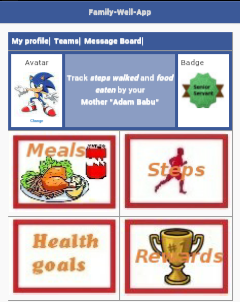
\epsfig{file=gameapp.png, height=3.15in, width=2.5in}
\caption{The main screen of the Family Health App}
\label{figure:gameapp}
\end{figure}

The Family Health App is a shared web-based user interface designed for use on a mobile phone, and to be operated by an intermediary member of a pair. The idea was to promote collaboration between members of each participating pair (team). It was expected by having one user interface then members of a pair will discuss what is happening on the app. We designed rules for interacting with gamification with an objective of having members of a pair contributing towards an overall success of a team. The objective was to have members of a pair collaborate in forming of, and achieving, their team's goal. 

Both versions of the app collect two types of personal health information: a step count measured by a pedometer on the phone, and diet, as entered by the participants. The steps recorded by the phone were automatically transferred every 30 minutes to the web app server, and could be manually pushed if the participants wanted an updated step count to immediately appear in the app.  The role of the intermediary was to help the beneficiary navigate the user interface and access the feedback.

\begin{figure}[H]
\centering

\epsfig{file=garden.png, height=1.8in, width=1.91in}
\caption{The number and size of plants in the garden increases as players get higher-ranked badges and record more fruits and vegetable consumption.}
\label{figure:botanical}
\end{figure}

\begin{figure}[H]
\centering
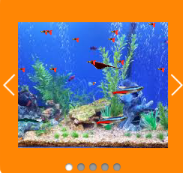
\epsfig{file=tank.png, height=1.8in, width=1.91in}
\caption{As with the botanical garden, the number and size of fish increases as players earn higher-ranked badges and record more fruit and vegetable consumption.}
\label{figure:tank}
\end{figure}

The gamified version of the app includes several additional features.  Each team is ranked on a leaderboard, based on frequency of app usage, step count, and their recorded eating habits. Teams are awarded sequential badges (e.g. queen, king) as they achieve specific goals, which is then displayed in the top right corner of the main screen (See Figure~\ref{figure:gameapp}). Another leaderboard displays the current badge for each team. As with the Fish'n'Steps app~\cite{lin2006:fish} or UbiFit garden app~\cite{klasnja2009:using}, achievements are also visualized in two ways, as a fish tank (Figure~\ref{figure:tank}) and as a botanical garden (Figure~\ref{figure:botanical}). The number of trees in the garden or fish in the tank was determined by the badge, the number of meals recorded, with a bonus given for meals that contain more fruits and vegetables. In addition, the system sends periodic SMS hints reminding intermediaries how to grow their gardens and fish tanks. For example:

``\emph{Tip of the day: Hey Kelvin, your fish in the aquarium need food to grow. You can only get enough points to buy fish food when you record every meal eaten by your Mother. You can get extra points if your Mother eats more fruits and vegetables..[This message was auto-generated by the Family Wellness App]}''. 

\section{Methodology}
We recruited study participants from low-income suburbs of Langa and Athlone in Cape Town, South Africa. We did a convenience sample, recruiting available parent-child pairs from the communities who were willing to commit to our study for six weeks. Our previous study had shown that when a pair consists of a parent working with his/her child, the child may assign more value to an intervention compared to when the beneficiary and intermediary are not related~\cite{katule2016:leveraging}. Putting value to a behaviour regulation can foster the \emph{identified and integrated regulations} during the process of behaviour internalization, as proposed by Ryan and Deci~\cite{ryan2000intrinsic}. Rationale for behaviour regulation is one of the facilitating social factors for  its internalization~\cite{deci1994facilitating}. 

A total of 14 adult participants with mean age of 44.2 (s.d. 10.0) years joined the study.  The youngest adult participant was 26 years old while the oldest was 60. Thirteen of these adult participants were female, since women were more easily accessible and eager to participate than men. While this gender imbalance is a limitation of our study, we argue that it does not necessarily affect the takeaways from our study. Sambasivan et al.~\cite{sambasivan2010} and Kumar and Anderson~\cite{kumar2015mobile} have pointed out that women in low-income communities are likely to suffer from constrained access to technology and digital information. A study focused on women, therefore, is likely to aid in exploring more complex social structures that influence technology access in related contexts. As a result, our study does not necessarily represent intermediated relationships in which the beneficiary is male, or even community benefits in which the target community is mixed gender. Therefore, the bias towards representation of women is still beneficial towards exploring complex social structures that influence the way technology is accessed in low income communities.

Each adult participant elected one of their children/grand-children to work with. The two members formed a pair and were required to work together in using the Family Health App to self-monitor the wellness of an adult member of a pair (a beneficiary user). The average age of intermediaries was 15.4 (s.d. 2.0) years. The youngest intermediary participant was 12 while the oldest was 20. The number of female and male intermediary participants/users were equal. Prior to joining the study the minor participants signed assent forms. Their guardians, the beneficiaries, signed the same forms as well as consent forms for themselves. All names used in this paper are pseudonyms.
  
We compared two versions of the Family Health App. The first version of the app was simply a logbook/journal supported by SMS reminders, that allowed each pair of users to self-monitor both steps graphs and nutrition components of food consumed by a beneficiary user. The second version added a game like component on the first version. The procedure of attaining rewards has already been explained in Section~\ref{gamfeatures} above. A full description of a gamified application together with its design process is explained by Katule et al.~\cite{katule2016:leveraging}.

\subsection{Experiment Design}
We used a within-group design where participants used both versions of the app to minimize the effect of confounding variables such as variation in motivation levels of beneficiaries and intermediaries, their technology operation skills, and their educational levels. Given the overhead and cost of recruitment, this approach helped to overcome the limitations of sample size. However, to minimize the impact of the learning effect on any experimental condition, each pair of users was randomly assigned to one of two experimental sequences. The LG group started with logbook and finished with gamification and the GL group did the opposite. Each group had seven pairs of users. We expect the learning effects from these two experimental conditions to cancel each other out.  However, our findings show that both groups were aware of both version of the app, which affected their behaviour regardless of which they used first. 

Our plan was to run the study with the participants spending three weeks with each version in October-November 2015. However, circumstances delayed execution of the midline assessment by one week. As a result, each group spent four weeks in the first phase.  While ideally we would have then proceeded to evaluate the second phase for an equivalent four weeks, this was impossible since many participants were traveling in late December for the holidays. These are some of the unforeseen challenges that can affect the rigor of a research design in resource-constrained environments.  

\subsection{Data collection and Analysis} 
Prior to data collection each pair was given an android phone (Samsung
GT-S5300) installed with both a native link to a web app and native pedometer app. The phones were supposed to be handled by adults. We allocated 1.3 GB of data to use for 6 weeks. Also each adult received ZAR 240 (\~USD20) as a compensation for transport and their time for the duration of the study. The data bundle was also an incentive to both members of a pair as they could use it for other purposes. 

Each participant was interviewed and administered an intrinsic motivation inventory (IMI) questionnaire at the beginning, midpoint (4 wks) and end (six weeks) of the study. However, the findings of this paper is based on one IMI questionnaire that was administered to intermediary users. We developed the IMI questionnaires with guidance of materials found on a \emph{Self-Determination Theory}\footnote{http://www.selfdeterminationtheory.org/intrinsic-motivation-inventory/} website which is maintained by researchers working on the theory including  Ryan and Deci~\cite{deci1985:intrinsic} whom were early pioneers in developing the theory. These questionnaires included sub-scales for the three basic psychological needs, together with perceived enjoyment and pretested in one of our early pilot studies~\cite{katule2016:leveraging}.  We also recorded and collected usage logs from the app.

Usage was measured by counting the number of sessions from each version of the system. A new session was defined as when an activity has been detected in the absence of any activity in the past one hour or more. We computed the relative number of sessions (normalized number of sessions) since the number of days on which pairs of users spent on a particular experimental condition differ between LG and GL group. For instance the LG group spent nearly four weeks in logbook and two weeks in gamification while the GL group spent four weeks in gamification and two weeks in logbook. Therefore, we use number of sessions per day which is obtained using Equation \ref{equation:sessions}. Usage comparison between logbook and gamification excluded four pairs of users because they had various technical problems that hindered their full participation in both experimental conditions. The list of pairs that were excluded and reasons for their exclusion are summarised on Table \ref{table:usageproblems}.
\begin{equation}
\label{equation:sessions}
y=t\SB{ni}/d\SB{ni}
\end{equation}
where:\emph{y} is number of sessions per day, \emph{t\SB{ni}} is total number of sessions for pair, \emph{n} in experimental condition, \emph{i}, and \emph{d\SB{ni}} is total number of days on which experimental condition i was available for pair n.
\begin{table}%[h!]
  \begin{center}
    \caption{Pairs with technical problems}
    \label{table:usageproblems}
	\begin{tabular}{|p{0.95cm}|p{0.75cm}|p{5.4cm}|}
		\hline
		Pair&Group&Problem\\
		\hline
		Pair A&GL &App not loading\\
		\hline
		Pair B&GL& Miss-allocation of data bundles.\\
		\hline
		Pair C & LG.& Pedometer never transmitted data.\\
		\hline
		Pair D & LG.& Pedometer stopped transmitting data.\\
	\hline
	\end{tabular}
  \end{center}
\end{table}
\section{Findings}
\subsection{Usage Trend} 
Figure \ref{figure:usagedailysessions} shows the usage of the app over six weeks for all participants. Peak usage occurs on the fifth day, when most participants started using the app, and decays quickly as the novelty effect dissipated. 
\begin{figure}[htbp]
  \centering
    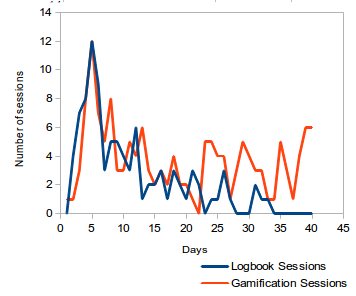
\includegraphics[width=0.32\textwidth]{scatter_daily_sessions.png}
    \rule{26em}{0.5pt}
  \caption{Total daily sessions from both conditions}
  \label{figure:usagedailysessions}
\end{figure} 
Comparison of usage between logbook and gamification (which excluded four pairs) showed that the log mean of number of sessions per day was significantly higher on gamification condition, M=0.459; SD=0.336, when compared to logbook condition, M=0.201; SD=0.196 with (t(9)= -2.6593; p= 0.0261; 95\% CI=-0.477 to -0.039). We used log mean because we transformed the original data to have a normal distribution shape on the differences between number of sessions per day. This finding suggests there was a significant increase in frequency of daily usage when pairs were in gamification condition.

\subsection{User Experience}
The use of the app was mostly controlled by intermediaries in proximate enabling and proximate translations~\cite{sambasivan2010}. Children were more skilled and familiar with using phones and smartphone apps than their parents. Hence, they did not face difficulties in familiarizing themselves with the intervention phones. Intermediaries operated the web interface and had face to face interactions to share feedback with their respective beneficiaries. We present user experience findings on factors that influenced usage of the app. We then present findings on effectiveness of gamification in fulfilling intermediaries' psychological needs of competence, relatedness, and autonomy.

\subsubsection{Mediators of App of Utilization}
Some observed factors that influenced use were phone effect, gamification, and help-seeking of beneficiaries.

\subsubsection*{\textbf{Reciprocation of unlimited access to the phone}}
A beneficiary user (parent) was a custodian of the intervention phone, meaning the phone was supposed to be carried around by a beneficiary user most of the time. However, the phone exchanged hands between a parent and child. This made some children utilize these phones for their own needs such social media and games. Children borrowed phones from their parents because: (1) they did not have phones at all or their phones were limited in functionality; and (2) to utilize available data bundle on phones. Children used data more often than their parents.

\userquote{\textbf{Siyamthanda}, female intermediary, 12 yrs} {``I had freedom because sometimes she left the phone with me and I was able to play games''}

\subsubsection*{\textbf{Effect of competition}}
Intermediaries competed with one another on the leader board and talked about their points whenever they physically met. In some cases, the competition fostered a close collaboration between members of participating pairs. For instance in the following excerpts, intermediaries appear to state explicit goals of winning against other teams to their team mates (beneficiaries) or attempt to encourage their respective beneficiary participants to do things that are advantageous in winning.

\userquote{\textbf{Kelvin}, male intermediary, 15 yrs} {``When I see other people trying to come above me [on the leader board]. I hand over the phone to my mum so she can walk more steps.''} 

\userquote{\textbf{Celine}, female intermediary, 16 yrs} {``I told my mom that me myself I want our team to have the highest points. Yes she said she is going to do that.''} 

The notion of competition also had an effect on intermediary users who were in logbook condition prior to being switched to gamification at a later stage. These users were already aware that they would be switched to gamification at some point; hence some of them took extra initiative to engage with the app during logbook condition with premise that once they were switched to gamification their activity would be reflected in the leaderboard. An example of this situation is that of an intermediary called  \emph{Siyamthanda}. She emphasized winning while her pair was still in the logbook phase. \emph{Kefiloe}, a female beneficiary, 26 years of age, narrated that scenario, \emph{``Most of the time she used to say, we must win this''}. 

At the same time, while some of the intermediaries exhibited interest in interacting with other users through the app, others were more concerned on dominating others in competitions:

\userquote{\textbf{Aziza}, a female beneficiary, 35 yrs} {``We [with Kelvin] were not talking to others because all we wanted was to win. We did not want them to know but they could see from the app.''}
 
Only two intermediaries tried to use social features on the app in order to interact with others. This entailed commenting on rewards from peers as highlighted below.

%\userquote{\textbf{Simon}, male intermediary, 15 yrs} {``Fish are increasing neh.[He commented this on a fish tank owned by Kelvin and his mother]''} 

\userquote{\textbf{Siyamthanda}, female intermediary, 12 yrs } {``Wow it shows that you are working hard, Clara\#2. [She congratulated a female intermediary called Clara for being on the second position on Fish tanks.]''} 

However, most conversation happened outside the app context, and therefore the relatedness brought by the app occurred in both the logbook and gamification conditions.

There were also incidences in which some pairs cheated in order to win. In one scenario, a mother and daughter took turns walking with the phone; they collaborated to accumulate more steps. 

\userquote{\textbf{Celine}, female intermediary, 16 yrs} {``I ask her how far did you walk?  She would say she walked very far. She tells me that I must have the phone to walk more steps. She would say, I got more more walking than you. She sometimes writes the steps on the page and she tells me yesterday I had more points [steps] than you''}   

The aforementioned scenario is an example of introjected regulation in self-monitoring behaviour of whereby participating members are influenced solely by competition with others.

\subsubsection*{\textbf{Requests from beneficiary users}}
Not all usage of the app was initiated by intermediaries. There were instances when intermediary users would use the app only after receiving requests from respective beneficiaries. These requests came through in both experimental conditions. Therefore, app usage was also as a result of fulfilling these help-seeking requests but at times they also served as reminders to intermediary users. For instance on the case of \emph{Kelvin} as explained by his mother.

\userquote{\textbf{Aziza}, female beneficiary, 35 yrs} {``I would remind him. Kelvin did you go to that app really? `Yes mum I am going to it now'. [This happened during gamification condition]''} 

We now look at how gamification fostered collaboration between intermediary and beneficiary users through requests by beneficiaries. These requests indicated a sense of collaborative ownership of the app. For beneficiaries that felt engaged with gamification, requests were phrased differently in the gamification condition than in the logbook condition. In logbook condition, the beneficiary user would use a statement like, `\emph{How am I doing on this?}' while beneficiaries that were interested in gamification would say, `\emph{How are we doing on this?}'. The former indicates authority while the latter indicates a more collaborative approach which is not authoritative and can promote autonomy of intermediaries.

\userquote{\textbf{Aziza}, female beneficiary, 35 yrs}{``I would always ask him [Kelvin] where are we. Are we first? And what badge do we have? Where are the others? How far is Simon [intermediary] then? How far is that one? `No mum we are on top. We are first. We are the champions' [during gamification].''} 

\userquote{\textbf{Samela}, female beneficiary, 43 yrs} {``I always start the conversation. Because I always want to make sure if he records because I can't use it. It was difficult for me to use it. [during logbook]''}

In these excerpts, the request made during the gamification condition is more inclusive. The request promotes collaboration, while the other one is a directive from a beneficiary user which does not consider whether an intermediary user is interested or not. In such directives, some intermediaries felt their autonomy was being violated as they felt that their parents were nagging them. For instance in a scenario of an intermediary participant in logbook condition, \textbf{Lunga}, a male aged 17 years from Langa, felt annoyed when his mother insisted they should get into the Family Wellness App while he was busy using social media through the intervention phone. Another situation happened to \textbf{Jennifer}, female aged 18 participant from Athlone, who also felt irritated by her mother's constant requests during logbook condition. She also felt the app was not that exciting: ``\emph{The app was okay at first but it started to get boring. You do not want to go into it any more. I think there will be some excitement now if the game comes in. When do we get the game?}''. 

\subsubsection{{SDT Support for Intermediaries}}  
Despite higher frequency of usage in gamification condition, the trend on average perceived enjoyment in logbook condition appears to be higher than in gamification condition for both age groups (age \textgreater = median(15.5) or \textless 15.5) (Figure \ref{figure:PE_Interm_App_exp_seq}). The reason behind this trend is that not all intermediary participants had a positive user experience on utilizing gamification. We observed two factors that contributed  to this. First, there were pairs that had usage problems as we have seen in Table~\ref{table:usageproblems} above. Among those four pairs, the user experience was severely bad for the intermediary users from pairs \emph{A} and \emph{C}. For pair A, the app demotivated the intermediary because it was not stable and always failing to load, resulting in termination of usage after two days. For pair C, the pedometer never transmitted a single reading to the server but this pair continued to use the app throughout the logbook condition. The intermediary user from this pair was close to the intermediary from pair D which experienced problems with pedometer that were less severe than those faced by pair C. As a result, the intermediary user from pair C continued to use the app in spite of the fact that the steps never got transmitted to the server, because they could directly compare steps in the pedometer, and for the novelty effect. Steps for pair C could still be viewed directly from a native pedometer app as raw numbers. The two intermediary participants from pairs C and D shared their progress about steps walked by their respective beneficiary users whenever they met. This explained why the pedometer problem did not affect the usage of the app by the intermediary user from pair C while in logbook condition. After pair C was switched to gamification, the inability of the pedometer to transmit steps to the server resulted to a negative user experience. This also happened to pair D but it did not affect much the motivation of this intermediary user as the pedometer was working until one week before switching of experimental conditions. Steps played a role in achievement of rewards. The intermediary user from pair C had invested a lot of effort with the expectation that their pair would be rewarded once they switched to gamification condition. This finding about expectations was shared by another intermediary user from pair E who was living close  to the two intermediaries from pairs C and D. She worried that the system was not fair because her peers had put in more effort but she was ahead of them did not understand why. She was referring to what she had observed during logbook condition,  therefore she was expecting the efforts of her peers to transmute into rewards after they were both switched to gamification condition. As the result the problems on pairs C, D had a multiplier  effect on the perceived enjoyment of this intermediary user from pair E; hence her motivation to use the gamified app and this affected her trust in the credibility of the gamified system.

\begin{figure}[htbp]
  \centering
    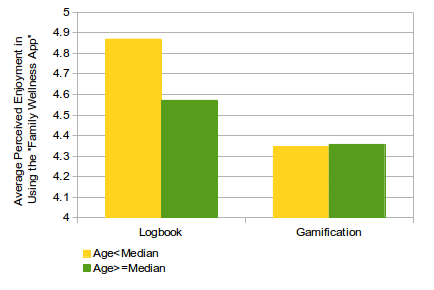
\includegraphics[width=0.35\textwidth]{PE_Interm_App_exp_seq.png}
    \rule{26em}{0.5pt}
  \caption{Intermediaries' average perceived enjoyment in using the app versus age group.}
  \label{figure:PE_Interm_App_exp_seq}
\end{figure}

Gamification also harmed motivation of two more intermediary users who never made any progress on badges. These users had used the app more often while in gamification compared to when they were in logbook but had both reported lower scores in competence when they were in gamification compared to when they were in logbook. The failure to progress in badges was attributed to less steps being detected because the respective beneficiary users were either not walking enough steps or not carrying the pedometer all the time; hence some of their steps could have been missed in detection. As badges were earned based on efforts done on both steps by beneficiary users and usage of app by the participating pair,  then absence of rewards harmed enjoyment of the two intermediary users in using the gamified app.

\begin{table}[h!]
  \begin{center}
    \caption{Comparison of 10 intermediaries' scores on sub-scales of perceived competence (PC), perceived autonomy (PA), and perceived relatedness (PR)}
    \label{table:imiwellnessinterm}
	\begin{tabular}{|L{0.6cm}|L{3cm}|L{3cm}|}
		\hline
		Mean &Logbook&Gamification\\
		\hline
		 \multirow{2}{*}{PC}&M=5.23; SD=1.02&M=5.96; SD=0.66\\\cline{2-3} 

		 &\multicolumn{2}{|l|}{t(9)=-3.495; p=0.0068 ; 95\% CI= -1.204 to -0.258} \\
\hline
		 \multirow{2}{*}{PA}&M=3.95; SD=0.86&M=3.96; SD=0.94\\\cline{2-3} 

		 &\multicolumn{2}{|l|}{t(9)= -0.027; p= 0.98; 95\% CI= -0.596 to 0.582} \\
\hline

		 \multirow{2}{*}{PR}&M=4.22; SD=0.63&M=4.37; SD=0.9\\\cline{2-3} 
		 &\multicolumn{2}{|l|}{t(9)= -0.719; p=0.49; 95\% CI= -0.622 to 0.322 } \\
\hline
	\end{tabular}
  \end{center}
\end{table}

We then compared the ability of the two versions of the app to afford the three basic psychological needs. In this comparison, we excluded pairs A, C, F, and G due to reasons stated above. The results for this comparison are shown in Table \ref{table:imiwellnessinterm}. Perceived competence of intermediaries in using our app was significantly higher in the gamified condition than in the logbook condition. This means a gamified system gave intermediary users challenges that motivated greater use of the app. There were no significant differences on both perceived autonomy and relatedness. 

\subsubsection{Unintended Internalization of Self-Monitoring}
There were some intermediaries who perceived benefits as an unintended effect. These intermediaries believed that the app had also helped them to eat healthy. Therefore, these individuals had put value in self-monitoring beyond just helping their parents to live healthy. 

\userquote{\textbf{Kelvin}, a male intermediary, 15 yrs} {``The app was very useful and very convenient. In many ways it helped me.  It shows me what I was eating and that. The information I was putting on the phone it was mostly hers. But we eat the same food and the same amount of food.''} 

Although there was some perceived value in self-monitoring of behaviour, regulation was not fully integrated as it still relied on external rewards. For instance, Kelvin, engaged with the app more often during gamification but his usage dropped in the logbook condition despite the fact that he appreciated the app could help him eat healthy. Therefore, this form of internalization can be categorized as identified regulation, since the behaviour is perceived as valuable but it is not fully integrated with individual's core beliefs and values.

\section{Discussion}
We discuss mediators of app usage such as availability of phones, the novelty effect, motivation of beneficiaries, and gamification. We also highlight strengths and weaknesses of gamification in the context of intermediated use.

\subsection*{\textbf{Use of intervention phones by intermediaries}}
In our prior work, beneficiaries who had no parent-child relationship dominated use of the intervention phone even in cases of familial relationships such as auntie and niece. These beneficiaries handed phones over to intermediaries only when help was needed~\cite{katule2016:leveraging}. In this study, all relationships between intermediaries and beneficiaries were parent-child bonds. Most parents were willing to trust their kids with their intervention phone. The phenomenon of sharing phones had an effect on mediating negotiation for interaction initiated by beneficiaries. Some parents let their kids access social media sites and games on the phones. In return, the kids fulfilled requests from their assigned beneficiaries.

Having access to a phone while providing help to beneficiary participants can be viewed as a reciprocation of benefits. Some intermediary participants had installed games and other apps on intervention phones. This non-prescribed use of devices or other technologies allocated for an intervention is an aspect of play that is a capability as it fosters motivation to participate in an intervention~\cite{Schwartz2013,ferr2015:play}. Therefore, sharing of phones enhanced the autonomy of intermediaries. This kind of sharing nurtured the permissive environment for help-seeking behaviours.  

Not all phones were accessible by intermediaries. Some beneficiaries maintained busy schedules and were less in contact with their kids, using the app less frequently. This brings another issue of maintenance of flow and spatial arrangement of users and technology. Having a technology in possession of beneficiaries can affect timely feedback to intermediaries in cases where beneficiaries are not in the vicinity. Timely feedback is an important aspect of cognitive flow. Flow in information design can be viewed as support for self-consciousness with the goal of fulfilling one's overall satisfaction~\cite{csikszentmihalyiflow}. This means timely reflection is important in flow. In this context, we have two layers of reflection of which one involves intermediaries, and another involves beneficiaries. It is challenging to support timely feedback in such a context. Therefore, spatial arrangement of technology may need further exploration.

\subsection*{\textbf{Novelty effect}}
Measuring the impact of gamification is complicated by the novelty effect. Koivisto and Hamari~\cite{koivisto2014demographic} found that perceived enjoyment and usefulness from gamification decline with use, suggesting that users might experience novelty effects from the service. In our case, the novelty effect appeared to influence both logbook and gamification. It explains the high usage at the beginning as shown in Figure \ref{figure:usagedailysessions}. Use of gamification appeared to be steady towards the end. However, there is a need to study longer term effects.

\subsection*{\textbf{Gamification}} 
Intermediary users were the main users of the application. Availability of game design elements increased the frequency of usage of the application. Gamification had created an ambiance of competitiveness among different pairs (teams). It also fostered collaboration between members of a team, with intermediaries contributing points through usage while beneficiaries contributed points through their footstep count. This fostered the bond between members of a pair, as has been found in similar studies that involve family members collaborating in health self-reflection~\cite{grimes2009toward,saksono2015spaceship}. However, in some pairs beneficiary users were less engaged with gamification; hence there was less collaboration between an intermediary and beneficiary. Motivation as the result of informal comparison of steps observed in our previous study~\cite{katule2016:leveraging}; was not common this time as beneficiaries had fewer direct interactions (face to face discussions) between themselves. We continue to emphasize the importance of such face to face interactions among different beneficiaries as it may be beneficial in engaging older beneficiaries with this type of intervention through social support from familiar participants.

On relatedness, intermediary participants had face to face interactions. This affected the ability to isolate the effect of social features provided by gamification, since these face to face interactions happened in both experimental conditions. The social features may be more important when teams are not collocated~\cite{lin2006:fish}. We also suggest that the aforementioned shortcoming was as the result of a small sample size. A study on social motivation to use gamification put an emphasis on the importance of having a larger network of users who are committed to the same goal because this has advantages of providing users with a better possibility of receiving recognition from others, get exposed to more social influence, and receive more reciprocal benefits from the use of gamification~\cite{hamari2013social}.

The main weakness of the gamified system is that it did not give users flexibility in defining how they wanted to participate in gamification. We had many motivational affordances under one system (leaderboard, badges, gardens and fish tank). It would have been interesting to give intermediary users an autonomy of selecting which part of the game they would like to participate. The idea of throwing so many features was meant to provide wider choices but it ended up overwhelming and confusing intermediary users. In addition to that, flexibility would have accommodated heterogeneity in users' personalities. The importance of tailoring persuasive games according to personalities of players has been emphasized~\cite{orji2013:tailoring}. Arteaga~\cite{arteaga2010:persuasive} designed a study involving motivating teenagers to exercise using persuasive health games, in which each player selected a game that matched their personality. It is also important to give users more autonomy in defining goals, and allow them to select the level of gamification and challenges that match their skills~\cite{zhang2008:motivational}. On our context, intermediaries did not have much power in formulation of goals as their performance relied on skills of beneficiaries (an ability to walk sufficient number of footsteps) to the great extent.

Exposing all intermediary users or pairs in general to competition among each other appeared to lessen the perceived value of the intervention as not all intermediaries were interested in inter-families competitions. Features that aimed at supporting task mastery climate (fish tanks, botanical gardens, badges) lost their importance on the presence of competition through a leaderboard. We argue that this restricted the gamified intervention not to reach identified and integrated regulations which are important modes of internalization close enough to intrinsic motivation. We also observed in the previous study~\cite{katule2016:leveraging},  there were examples of users who appeared to constantly focus on winning against other teams, one of them admitted that fish in their team's tank were medium sized as he was not really feeding them, meaning that he was not carrying out the task of recording food eaten by his beneficiary more often. Researchers have also cautioned that competitions in health settings should be examined with some degree of sensitivity as it can lead to negative consequences~\cite{grimes2009toward}. It has been emphasized that supporting of  challenges should be done on the level of \emph{task mastery climate} rather than on competition that has \emph{ego involved climate} as the  former foster intrinsic motivation while the latter can harm it~\cite{saksono2015spaceship}. When there is ego involved, participants may do things just to maintain their self-worth, and this is equivalent to introjected regulation as postulated by organismic integration theory (a sub-theory of SDT)\cite{ryan2000:self}. In introjected regulation individuals don't see any value in regulating a behaviour (i.e. intermediaries assisting their parents in self-monitoring tasks) rather they perform it merely for the purpose of outdoing others or maintaining their social status. 

\section{Conclusions}
The study has demonstrated that gamification increased perceived competence of intermediary users and fostered both collaboration and relatedness of members of a participating pair. A further exploration is needed on utilization of features that promote task mastery climate and also the best way to design inter-families' competitions without harming intrinsic motivation of participating pairs. We recognize that there were limitations in supporting self reflection for both members of a participating pair, future studies need to explore an optimal spatial arrangement of users and technology in order to support cognitive flow for each member of a participating pair. Also considering intermediaries as passive consumers of information lessens engagement of intermediaries.  Since the findings indicated that intermediaries can also benefit from such health information, therefore, researchers should explore the effect of integration of intermediaries' wellness data on engagement of intermediaries.

Another shortcoming of this study was a limited sample size; hence it fails to take advantage of network effect which is a mediator for exploiting the power of gamification. Apart from a small sample size, we also faced a myriad of challenges such as intermittent connectivity that affected the generalizability of these findings. Ramachandran et al~\cite{ramachandran2010research} have highlighted how doing research in ICTD contexts poses challenges to the rigor of research design. Our study is one step towards exploring the feasibility of engaging intermediaries through gamification. Future work can look into the aforementioned unexplored issues. 

%ACKNOWLEDGMENTS are optional 
\section{Acknowledgments} 
This work would have not been possible without the generous funding of the Telkom Centre of Excellence (CoE) and the HPI Research School at University of Cape Town.  We also thank our reviewers for valuable feedback on the manuscript.  We give special thanks to Neha Kumar for going above and beyond in shepherding this paper.

%\section{Acknowledgments} 

%
% The following two commands are all you need in the
% initial runs of your .tex file to\ref{equation:sizetrees}
% produce the bibliography for the citations in your paper.
%small{
\bibliographystyle{abbrv}
\bibliography{sigproc} %} % sigproc.bib is the name of the Bibliography in this case
% You must have a proper ".bib" file
%  and remember to run:
% latex bibtex latex latex
% to resolve all references
%
% ACM needs 'a single self-contained file'!
%
%APPENDICES are optional
%\balancecolumns

\end{document}